\documentclass{standalone}
\usepackage{graphicx}	
\usepackage{amssymb, amsmath, amsthm}
\usepackage{color}

\usepackage{tikz}
\usetikzlibrary{intersections, backgrounds}

\definecolor{light}{RGB}{220, 188, 188}
\definecolor{mid}{RGB}{185, 124, 124}
\definecolor{dark}{RGB}{143, 39, 39}
\definecolor{highlight}{RGB}{180, 31, 180}
\definecolor{gray10}{gray}{0.1}
\definecolor{gray20}{gray}{0.2}
\definecolor{gray30}{gray}{0.3}
\definecolor{gray40}{gray}{0.4}
\definecolor{gray60}{gray}{0.6}
\definecolor{gray70}{gray}{0.7}
\definecolor{gray80}{gray}{0.8}
\definecolor{gray90}{gray}{0.9}
\definecolor{gray95}{gray}{0.95}

\begin{document}

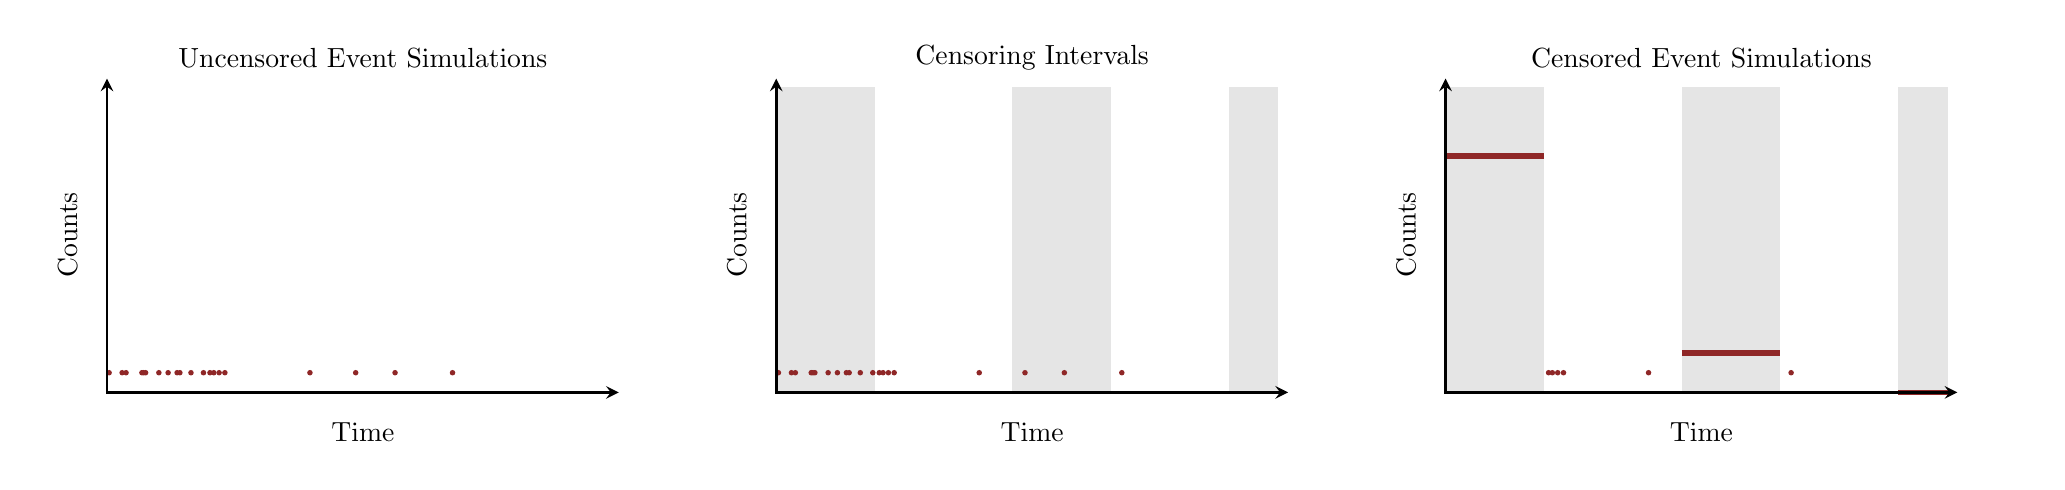
\begin{tikzpicture}[scale=0.25]
  \begin{scope}[shift={(0, 0)}]
    \draw[white] (-17, -11.5) rectangle (17, 10.5);
    
    \node at (0, 9) { Uncensored Event Simulations };
    
    \foreach \t in {0.110, 0.771, 0.970, 1.776, 1.863, 1.963, 2.636, 3.107, 
                    3.563, 3.704, 4.268, 4.903, 5.233, 5.426, 5.697, 5.991, 
                    10.311, 12.635, 14.635, 17.554} {
      \fill[color=dark] (\t - 13, -8 + 1) circle (4pt);
    }
  
    \draw [->, >=stealth, line width=1] (-13, -8) -- +(26, 0);
    \draw [->, >=stealth, line width=1] (-13, -8.058) -- +(0, 16);
    \node[] at (0, -10) { Time };
    \node[rotate=90] at (-15, 0) { Counts };
  \end{scope}

  \begin{scope}[shift={(34, 0)}]
    \draw[white] (-17, -11.5) rectangle (17, 10.5);
    
    \node at (0, 9) { Censoring Intervals };
    
    \fill[gray90] (-13, -8) rectangle (-8, 7.5);
    \fill[gray90] (-1, -8) rectangle (4, 7.5);
    \fill[gray90] (10, -8) rectangle (12.5, 7.5);
    
    \foreach \t in {0.110, 0.771, 0.970, 1.776, 1.863, 1.963, 2.636, 3.107, 
                    3.563, 3.704, 4.268, 4.903, 5.233, 5.426, 5.697, 5.991, 
                    10.311, 12.635, 14.635, 17.554} {
      \fill[color=dark] (\t - 13, -8 + 1) circle (4pt);
    }
  
    \draw [->, >=stealth, line width=1] (-13, -8) -- +(26, 0);
    \draw [->, >=stealth, line width=1] (-13, -8.058) -- +(0, 16);
    \node[] at (0, -10) { Time };
    \node[rotate=90] at (-15, 0) { Counts };
  \end{scope}
  
  \begin{scope}[shift={(68, 0)}]
    \draw[white] (-17, -11.5) rectangle (17, 10.5);
    
    \node at (0, 9) { Censored Event Simulations };
    
    \fill[gray90] (-13, -8) rectangle (-8, 7.5);
    \fill[gray90] (-1, -8) rectangle (4, 7.5);
    \fill[gray90] (10, -8) rectangle (12.5, 7.5);
  
    \draw [-, >=stealth, line width=2, dark] (-13, -8 + 12) -- (-8, -8 + 12);
    \draw [-, >=stealth, line width=2, dark] (-1, -8 + 2) -- (4, -8 + 2);
    \draw [-, >=stealth, line width=2, dark] (10, -8) -- (12.5, -8);
  
    \foreach \t in {5.233, 5.426, 5.697, 5.991, 
                    10.311, 17.554} {
      \fill[color=dark] (\t - 13, -8 + 1) circle (4pt);
    }
  
    \draw [->, >=stealth, line width=1] (-13, -8) -- +(26, 0);
    \draw [->, >=stealth, line width=1] (-13, -8.058) -- +(0, 16);
    \node[] at (0, -10) { Time };
    \node[rotate=90] at (-15, 0) { Counts };
  \end{scope}
   
\end{tikzpicture}

\end{document}  